\chapter{Problem Domains}\label{ch:problems}
\chapterquote{But oversimplifying the real world is a bad idea---and unfortunately, that’s exactly what the Primitive Mind likes to do.}{Tim Urban}

In this thesis, we consider several diverse, safety-critical, real-world problems.
Broadly, the domains we study focus on the fields of aviation, robotics, and geological sustainability.

\section{Aviation: Safety-Critical Systems}
A culture of safety is ingrained in the field of aviation \cite{oster2013analyzing}.
Lessons regarding safety are often shared among competing aviation companies, with a collective objective of increasing safety throughout the field.
Stakeholders from industry, government, and academia come together to discuss safety concerns and develop solutions for the broader community \cite{do178c}.
In our work, we study three different safety-critical aviation systems.

\subsection{Aircraft Collision Avoidance}
Aircraft collision avoidance systems (CAS) are decision support tools designed to alert pilots when an immediate collision is imminent and provide recommended guidance to mitigate midair collisions \cite{kochenderfer2012next}.
In our work, we apply our methods to a simplified CAS problem, modeled after ACAS X \cite{do358a}:~the successor to the \textit{traffic alert and collision avoidance system} (TCAS) \cite{do185b}, mandated worldwide on all large aircraft~\cite{tcas2011introduction}.
Shown in \cref{fig:cas} (adapted from \textcite{dmbook}), the CAS state space consists of the relative altitude $h_\text{rel}$ in meters, relative vertical rate $\dot{h}_\text{rel}$ in meters per second, the previous action $a_\text{prev}$ in meters per second, and the time to collision $t_\text{col}$ in seconds.
The \textit{ownship} is our own aircraft making the decisions and the \textit{intruder} is a non-cooperative intruding aircraft.
The objective is to provide climb or descend maneuver guidance by issuing $5$ m/s, $-5$ m/s, or $0$ m/s relative vertical rate change actions.

\begin{figure}[t!]
    \centering
    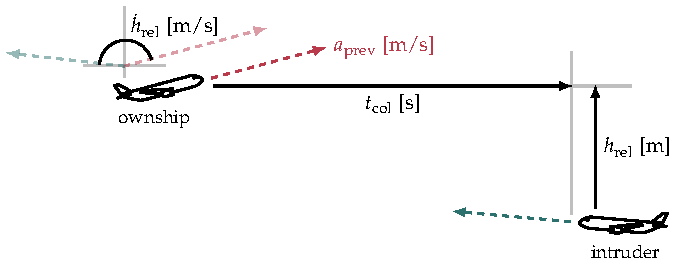
\includegraphics[width=0.75\textwidth]{diagrams/background/cas}
    \hspace*{1cm}
    \caption{State space of the aircraft collision avoidance system.}
    \label{fig:cas}
\end{figure}


\subsection{Autonomous Runway Detection}
To support the development of safe autonomous aircraft, subsystems such as camera-based runway detectors help localize the autonomous aircraft on an approach to land \cite{gautam2014survey}.
Companies such as Airbus (through their A$^3$ subdivision) \cite{airbus2019wayfinder} and Xwing (now part of Joby Aviation) \cite{durand2023formal} have been developing vision-based runway detection systems that rely on complex neural networks to detect and track the edges of the runway.
The runway information is used to augment GPS/INS localization information during landing.
Validating the runway detection system is an important step not only for system safety before deployment, but to help in the certification process of machine learning components for autonomous flight \cite{durand2023formal}.
The state space for runway detection systems consists of all possible RGB images of runways the system will encounter.
Thus, validating in simulation over a parametric space (e.g., glide slope angle, distance to runway, time of day, weather, etc.) is important to study to reduce the dimensionality of the near-infinite possible runway images.
It is important that high-fidelity simulators generate the runway images to ensure that the system sees representative examples of images it would encounter during deployment.

\subsection{Airborne Wildfire Suppression}
Wildfire incident commanders are tasked with processing continuous streams of information to enable effective decision making when allocating resources to mitigate the spread of and suppress wildfires \cite{pyne1996introduction}.
Recently, the development of decision support tools to provide recommendations to incident commanders has been studied to help offload planning where to place resources to reduce the over-saturation of information \cite{griffith2017automated}.
Airborne wildfire suppression systems are tools designed to recommend approximately optimal placements of aerial suppression resources by planning over the uncertainty in the wildfire spread.
Such tools need to consider the potential catastrophic damage to land and minimize the risk of the wildfire spreading to populated areas.
The state space consists of all currently burning areas, the remaining fuel levels (as a function of the terrain), elevation, and the angle and speed of the current winds.
The suppression agent can make aerial resource placements to suppress the wildfire with some probability of complete suppression and the environment transitions based on models of the wildfire spread \cite{boychuk2009stochastic}.
The goal is to quickly suppress the wildfire while simultaneously protecting nearby populated areas. 


\section{Robotics: Safety-Critical Systems}
Robots have been used as autonomous systems in cases deemed too risky for humans \cite{guiochet2017safety}.
Our work studies robotics systems dealing with localization, navigation, and exploration.

\subsection{Robot Localization and Navigation}
When robots operate in real-world environments, they require sensor measurements to observe the world around them.
Using these measurements, robots can localize their position to enable better performance in their primary objective, e.g., navigate to a goal.
A common benchmark used to study sequential decision making algorithms is the \textit{light dark} problem \cite{platt2010belief}, consisting of a simplified 1D environment where a robot receives noisy observations in the \textit{dark} region, and more accurate observations in the \textit{light} region.
The task of the robot is to first localize its position in the light region, and then navigate to a goal.
Considered an information gathering problem, this problem deals with planning over long horizons to get to the light region to localize, delaying the primary goal.

\subsection{Robot Exploration}
Robots have also been used to explore unknown or dangerous environments, such as the lunar surface \cite{balaban2020health}.
Another common benchmark for sequential decision making is the \textit{rock sample} problem introduced by \textcite{smith2004heuristic}.
In rock sample, an autonomous agent operates in an $n \times n$ grid and is tasked with collecting information about the $k$ rocks in the environment.
Certain rocks are marked \textit{good}, while others are marked \textit{bad}.
The objective is to collect information about all of the good rocks, while avoiding any penalties if observing the bad rocks.
Rock sample is a scalable problem in $n$ and $k$, allowing researchers to study more challenging, high-dimensional problems.


\section{Geological Sustainability: Safety-Critical Systems}
Geological sustainability plays a crucial role in mitigating the impacts of climate change through systems like carbon capture and storage \cite{boothandford2014carbon}, geothermal energy production \cite{aikin2019enhanced}, and critical mineral exploration and discovery \cite{mern2023intelligent}.
Many geological systems evolve over long time horizons and present significant challenges due to limited subsurface observability and high uncertainty.
In these safety-critical scenarios, it is often challenging to balance information gathering with preserving safety of infrastructure or human life.

\subsection{Critical Mineral Exploration}
As we move away from reliance on fossil fuels, the need for rare Earth metals---such as copper and lithium \cite{sovacool2020sustainable}---becomes increasingly important.
Recent research has proposed the use of decision support tools to automate the selection of drilling locations in critical mineral exploration and discovery problems \cite{mern2023intelligent}.
In the critical mineral exploration problem, an agent selects drilling locations to better understand the uncertain subsurface through bore hole measurements.
Using prior models developed by geologists, the agent can collect information about the subsurface and use this information to make a final \texttt{mine} or \texttt{abandon} decision regarding the economic value of the project.
Safety, in this case, can be considered either as minimizing the risk of induced seismicity \cite{gibowicz2009seismicity} or constraints on the risk of exceeding the project's budget.
In more recent work, detailed in \cref{ch:ivae}, the use of passive cosmic-ray muon tomography \cite{lechmann2021muon} has been developed as an alternative means to collect subsurface information about an ore body or intrusion.


\subsection{Safe Carbon Capture and Storage}
To help offset CO$_2$ emissions, carbon capture and storage (CCS), or \textit{carbon sequestration}, is a method to capture CO$_2$ from the atmosphere and store it in underground porous rock formations \cite{boothandford2014carbon}.
\textcite{wang2023optimizing} proposed a formal CCS problem formulation, enabling direct application and study of sequential decision making algorithms.
In the CCS problem, an agent makes decisions on where to drill to inject CO$_2$ and builds knowledge of the CO$_2$ plume migration through information gathering actions.
Safely storing CO$_2$ is important as improper understanding of the subsurface may lead to concentrated CO$_2$ leakage back out into the atmosphere \cite{lee2018co2}.
We apply our methods to a 2D problem formulation of safe CCS developed by \textcite{corso2022pomdp}.


\section{Broader Applications}

Across all domains presented in this chapter, a common theme is the need to make sequential decisions under uncertainty with only partial information.
The POMDP framework provides a principled way to model these problems, allowing autonomous systems or decision support tools to explicitly reason about uncertainty and risk.
The safety-critical domains studied in this thesis were chosen to reflect a range of problem sizes, time horizons, and failure modes.
Although we focus on aviation, robotics, and geological systems, many other safety-critical applications---including healthcare \cite{zhang2022diagnostic}, autonomous vehicles \cite{wray2021pomdps}, disaster response \cite{sankar2020evacuate}, and financial planning \cite{cho2017robust}---share these characteristics.
Extending this work to such domains requires scalable planning under uncertainty, efficient belief representation, and domain-specific safety constraints---challenges our contributions are designed to address.
